\chapter{Avaliação}
\label{chp:evaluation}

Neste capítulo, será mostrado o processo de avaliação utilizado para verificar se os objetivos previstos foram alcançados. Espera-se que com a criação de rotas de pontos turísticos o usuário possa visitar a maior quantidade de lugares dentro da sua rota de origem e destino. Para isso, os experimentos aqui utilizam o OpenStreetMap e Google Maps como fonte de dados, tanto de usuário, tanto dos domínios de pontos de interesses. A avaliação consiste em comparar as combinações de diferentes tipos de metadados, utilizando os algoritmos de sistemas de recomendações. Também serão apresentados neste capítulo os detalhes da metodologia utilizada para desenvolver e avaliar este trabalho, bem como o conjunto de dados utilizados durante os experimentos. Em seguida, são apresentadas as métricas utilizadas na avaliação e os resultados obtidos. Por fim, é feita uma discussão e apresentados pontos de melhoria.

\section{Metodologia}

Os testes realizados para a avaliação tem por objetivo mostrar que é possível recomendar pontos turísticos de acordo com as preferências do usuário. Além disso, os testes exibem a precisão das recomendações, de acordo com as atribuições escolhidas para análise e o modelo de recomendação.

Para avaliar os modelos serão realizadas comparações, variando de acordo com os dados que cada um dos modelos utilizam para gerar as recomendações. No caso do modelo \textit{Item Similarity}, diferenciou-se o tipo de similaridade entre \textit{Jaccard}, \textit{Cosine} e \textit{Pearson Correlation}, mencionados em \ref{subsubsec:similarity_metrics}. Já no caso do \textit{Item Content}, intercalou-se entre os atributos da base de dados de itens. Considerando as informações do ID do item, as combinações foram: somente uma categoria; uma ou mais categorias; somente localização; localização e uma categoria; localização e uma ou mais categorias; nome; nome e somente uma categoria; nome e uma ou mais categorias; nome e localização; nome, somente uma categoria e localização; e todas as atribuições. 

Para os testes, utilizou-se o processo de \textit{Cross-Validation}, criando conjuntos de treino e de teste. Utilizando o conjunto de treino, o modelo é treinado e testa-se com os exemplos do conjunto de teste. Depois, diferentes conjuntos de treino e de teste são selecionados para iniciar o processo de treino e teste novamente, sendo repetido $k$ vezes \citep{Ricci:2010:RSH:1941884}. Com os arquivos e os modelos mencionados anteriormente, todos os testes foram realizados com a biblioteca GraphLab\footnote{https://turi.com/}. Para medir a precisão de cada uma das comparações, foram utilizadas as métricas \ac{rmse}, \textit{Precision}, \textit{Recall} e F-\textit{Score}.


\section{Conjunto de Dados}

Os testes foram executados com dados oriundos de diversas fontes. Primeiramente, foram coletados dados do OpenStreetMap\footnote{https://www.openstreetmap.org} para obter informações sobre pontos de interesse relacionados a turismo da cidade de Salvador e quais são suas categorias. Depois, foram coletados dados do Google Maps para obter \textit{reviews} dos locais. Devido a limitação da API do Google, a ferramenta só disponibiliza as 5 últimas avaliações de cada ponto de interesse. Portanto, cada local tem, no máximo, 5 \textit{ratings}. Além disso, alguns locais tem mais de uma categoria. No total, o banco de dados foi composto de 178 usuários, 52 pontos de interesse de 12 tipos diferentes e 227 avaliações, como pode ser visto na Tabela \ref{tab:dataset_Salvador}

\begin{table}[H]
	\centering
	\caption{Conjunto de Dados de POI da cidade de Salvador.}
	\label{tab:dataset_Salvador}
	\begin{tabular}{|c|c|}
		\hline
		\multicolumn{2}{|c|}{\textbf{Conjunto de Dados}} \\ \hline
		Usuários                  & 178                   \\ \hline
		Pontos de Interesses      & 52                   \\ \hline
		Categorias de POI         & 12                 \\ \hline
		Avaliações                & 227                 \\ \hline
	\end{tabular}
\end{table}


Existem várias técnicas de \textit{Cross-Validation}, aqui foi utilizada a técnica através da porcentagem dos dados que devem ser mantidos para treino e para teste, devido a pouca quantidade de avaliações no conjunto de dados. Neste projeto, a proporção que foi de 80\% para o conjunto de treino e 20\% para o conjunto de testes para criar o conjunto de validação. Os algoritmos utilizados foram os de \textit{Item Similarity}, ou Similaridade de Itens e \textit{Item Content}, em português Conteúdo dos Itens.

\section{Métricas de Avaliação}

Em um sistema de recomendações, é fornecido ao usuário uma lista de recomendações. ele pode avaliar os itens como relevantes ou não relevantes. Essas métricas são conhecidas como Precisão (\textit{Precision}, em inglês) e \textit{Recall}. São utilizadas na recuperação de informação e úteis para avaliar a qualidade de um modelo de recomendação \citep{ParraSahebi2013}. Precisão é a fração dos itens recomendados que são relevantes \citep{Manning:2008:IIR:1394399}, sendo definida como

\begin{equation}
    precision = \frac{itens~relevantes~recomendados}{itens~na~lista}~~,
\end{equation}

Recall é definida como a fração de recomendações relevantes que são apresentadas para o usuário:

\begin{equation}
    recall = \frac{itens~relevantes~recomendados}{itens~relevantes}~~,
\end{equation}

\subsection{Precisão em n (\textit{P@n})}

As métricas de avaliação irão considerar apenas os itens do topo, chamados de Top-N recomendações, e são normalmente apresentados como precisão em n (\textit{P@n}). Isso acontece pois o número de itens recomendados em uma lista pode ser muito alto, dependendo do modelo de recomendação e do tamanho do conjunto de dados. \textit{P@n} é utilizado para avaliar o sistema no contexto de um único usuário. A equação de \textit{P@n} que mede a relevância dos $n$ primeiros itens da uma lista é:

\begin{equation}
    P@n = \frac{r}{n}~~,
\end{equation}

no qual $n$ é o número de itens retornados e $r$ é o número de itens considerados relevantes e retornados até a posição $n$ da lista.

\subsection{Recall em n (\textit{R@n})}

Assim como a precisão, Recall também considera apenas os itens do topo, os Top-N recomendações. A equação de \textit{R@n} que mede a proporção de itens relevantes que foram recomendados de entre todos os relevantes é:

\begin{equation}
    R@n = \frac{e}{n}~~,
\end{equation}

no qual5.3ondené $n$ é o número de itens relevantes e recomendados e $e$ é o número de itens relevantes até a posição $n$ da lista.

Tanto o resultado do \textit{Precision}, tanto o resultado do \textit{Recall} variam entre 0 e 1. Quanto mais alto for o valor, melhor é a performance do modelo. Se o valor da \textit{Precision} for 1, significa que todos os itens recomendados são relevantes, no entanto, não se sabe se todos os relevantes foram recomendados. Caso o valor do \textit{Recall} seja 1, mostra que todos os itens relevantes foram recomendados, mas não se sabe quantas recomendações não são relevantes \citep{morais2012sistemas}.

Essas duas medidas são inversamente relacionadas e sozinhas não permitem avaliar completamente o sistema. Aumentando o número de itens recomendados, o \textit{Recall} tem tendencia a aumentar porque maior é a probabilidade de os itens relevantes serem selecionados, assim como a \textit{Precision} diminui. Por isso, escolheu-se uma outra medida que incremente na análise da avaliação \citep{morais2012sistemas}.

\subsection{F1-\textit{Score}}

F1-\textit{Score} é a média ponderada de \textit{Precision} e \textit{Recall}, ou seja, é o equlibrio entre a precisão e o recall. Essa medida é definida pela seguinte expressão:

\begin{equation}
    F_1 = 2 \cdot \frac{precision \cdot recall}{precision + recall}.
\end{equation}

Assim como a \textit{precision} e o \textit{recall}, F1 varia igualmente entre 0 e 1. Quanto maior for o valor, melhor é o resultado da avaliação. Como neste trabalho está sendo utilizado dois modelos de recomendação e verificando os seus resultados, está medida vai ser utilizada principalmente para a avaliação de performance do algoritmo de recomendação.

\subsection{\textit{Root Mean Square Error (RMSE)}}

Para mensurar como está a acurácia do sistema de recomendação, é preciso utilizar além da precisão e da cobertura, que classificam os itens como boas ou más recomendações, é possível utilizar de métricas para averiguar a classificação dos itens em uma determinada escala \citep{Jannach:2010:RSI:1941904}. Nesse projeto, foi utilizado o \textit{RMSE}. Basicamente, o \textit{RMSE} calcula o desvio entre as avaliações previstas e as reais avaliações porém coloca mais ênfase no maior desvio \citep{Jannach:2010:RSI:1941904}. A equação de \textit{RMSE} é:

\begin{equation}
    RMSE = \sqrt{\frac{1}{N} \sum_{i=1}^{N} (p_i - r_i)^2}
\end{equation}

, supondo que $p$ e $r$ são vetores de tamanho $N$ e que $r$ contém as reais avaliações e $p$ as avaliações previstas. O valor do \ac{rmse} é o mesmo do atributo escolhido para ser a variável dependente. Tanto no \textit{Item Content}, tanto no \textit{Item Similarity}, a variável escolhida é o valor da nota atribuído ao item pelos usuários, que varia entre 1 a 5.

\section{Resultados}

Para avaliar os resultados foram utilizadas as seguintes métricas de avaliação:

\renewcommand{\labelenumi}{\roman{enumi})}
\begin{enumerate}
    \item \acfi{rmse}, o desvio entre as avaliações previstas e as reais;
    \item Precisão, que calcula o percentual de itens recomendados que são relevantes;
    \item Recall, que calcula o percentual de itens relevantes que foram recomendados;
    \item F1-\textit{Score}, a média ponderada entre precisão e recall.
\end{enumerate}

Os valores de cada métrica estão na Tabela \ref{tab:results_item_similarity}, que mostra os resultados para o modelo de recomendação \textit{Item Similarity} de acordo com os tipos de similaridade; a Tabela \ref{tab:results_item_content}, que apresenta os resultados para o modelo \textit{Iem Content}, de acordo com os atributos de itens que foram utilizados em cada teste. A Tabela \ref{tab:all_results} mostra os resultados dos dois modelos. Na identificação, foram utilizadas as seguintes convenções: [IS-XX] para os testes com \textit{Item Similarity} e [IC-XX] para os testes com \textit{Item Content}, no qual os números são de acordo com a coluna \textit{ID} das Tabelas \ref{tab:results_item_similarity} e \ref{tab:results_item_content}.

\begin{table}[H]
    \centering
    \caption{Resultados para \textit{RMSE}, \textit{P@10} e \textit{R@10} no modelo \textit{Item Similarity}.}
    \label{tab:results_item_similarity}
    \begin{tabular}{|c|c|c|c|c|c|}
        \hline
        \textit{ID} & 
        \textit{Tipo de Similaridade} & 
        \textit{RMSE} & 
        \textit{P@10} & \textit{R@10} & F1-\textit{Score} \\ \hline
        01 & Jaccard & 4.42010 & 0.01250 & 0.11250 & 0.02250 \\ \hline
        02 & Cosine & 4.35065 & 0.01250 & 0.11250 & 0.02250 \\ \hline
        03 & Pearson Correlation & \textbf{1.37313} & \textbf{0.03000} & \textbf{0.25000} & \textbf{0.05357} \\ \hline
    \end{tabular}
\end{table}

\subsection{\acfi{rmse}}

A métrica \acl{rmse} foi utilizada para medir o desvio de erro do algoritmo. Analisando os resultados obtidos pelo \ac{rmse} nas tabelas, conclui-se que existe um desvio muito grande entre as avaliações previstas e as reais.

No nosso projeto, essa métrica é avaliada da seguinte forma: no caso do modelo \textit{Item Similarity}, é esperado que o sistema de recomendação sugira pontos turísticos semelhantes ao que o usuário já avaliou, com base em usuários em comum. Ou seja, se um usuário visitou o Museu Náutico da Bahia, a preferência é que sejam recomendados pontos turísticos semelhantes com outros itens da base de dados para o usuário em questão. Já no modelo \textit{Item Content}, a semelhança entre os itens recomendados é determinado pelo conteúdo desses itens, ao invés de usar padrões de interação do usuário para calcular a similaridade. Voltando ao exemplo do Museu Náutico da Bahia, que se encaixa na categoria museu, este modelo irá recomendar pontos turísticos com a mesma categoria, no caso, irá sugerir outros museus.

No modelo \textit{Item Similarity}, o que menos teve erros foi o modelo \textit{Pearson}, com o valor de 1.37313 e o maior foi o do Jaccard, com 4.42010. Já no \textit{Item Content}, o menor (mas não o melhor), foi quando utilizou o atributo Localização e o pior foi o com a característica Nome. Este resultado era de se esperar, pois a base de dados ainda está muito incipiente: existe poucos usuários com mais de uma avaliação em diferentes itens, o que compromete com os resultados obtidos. Quanto mais usuários com mais e mais avaliações, melhor será a predição e a recomendação para futuros usuários.

\subsection{P@10 e R@10}

O P@10 considera a precisão dos dez primeiros itens da lista, pontuando mais os acertos nos dez primeiros itens. Analisando os resultados, no modelo \textit{Item Similarity}, este valor foi igual tanto no \textit{Jaccard} tanto no \textit{Cosine}. O melhor valor foi obtido pelo tipo de similaridade \textit{Pearson Correlation}. No caso de \textit{R@10}, o melhor resultado foi obtido também no tipo de similaridade \textit{Pearson Correlation}, ligeiramente maior comparado a \textit{Cosine} e \textit{Jaccard}, estes que tiveram o mesmo valor.

\begin{table}[H]
    \centering
    \caption{Resultados para RMSE, P@10 e R@10 no modelo \textit{Item Content}.}
    \label{tab:results_item_content}
    \begin{tabular}{|c|p{15em}|c|c|c|c|}
        \hline
        \multicolumn{1}{|>{\centering}c|}{\textit{\textbf{ID}}} &
        \multicolumn{1}{>{\centering}p{15em}|}{\textit{\textbf{Atributos de Itens}}} &
        \multicolumn{1}{>{\centering}c|}{\textit{\textbf{RMSE}}} &
        \multicolumn{1}{>{\centering}c|}{\textit{\textbf{P@10}}} &
        \multicolumn{1}{>{\centering}c|}{\textit{\textbf{R@10}}} &
        \multicolumn{1}{>{\centering}c|}{\textit{\textbf{F1-\textit{Score}}}} \\ \hline
        01 & Somente uma categoria & 4.06223 & 0.02750 & 0.23750 & 0.04929 \\ \hline
        02 & Uma ou mais categorias & 4.09162 & 0.03500 & 0.30000 & 0.06269 \\ \hline
        03 & Localização & \textbf{3.41135} & 0.04000 & 0.31875 & 0.07108 \\ \hline
        04 & Localização e somente uma categoria & 3.50065 & 0.05000 & 0.43750 & 0.08974 \\ \hline
        05 & Localização e uma ou mais categorias & 3.56493 & \textbf{0.05250} & \textbf{0.47500} & \textbf{0.09455} \\ \hline
        06 & Nome & 4.39682 & 0.03000 & 0.26875 & 0.05397 \\ \hline
        07 & Nome e somente uma categoria & 4.18395 & 0.04250 & 0.37500 & 0.07635 \\ \hline
        08 & Nome e uma ou mais categorias & 4.21318 & 0.04750 & 0.42500 & 0.08545 \\ \hline
        09 & Nome e localização & 3.64087 & 0.04250 & 0.33125 & 0.07533 \\ \hline
        10 & Nome, localização e somente uma categoria & 3.64233 & 0.04750 & 0.41250 & 0.08519 \\ \hline
        11 & Todos os atributos & 3.72535 & \textbf{0.05250} & \textbf{0.47500} & \textbf{0.09455} \\ \hline
    \end{tabular}
\end{table}

No \textit{Item Content}, o \textit{Precision} e o \textit{Recall} tiveram uma melhora de aproximadamente 75\% e 90\% respectivamente, comparado entre o maior valor do \textit{Item Similarity} e do \textit{Item Content}. O maior valor alcançado pelo \textit{P@10} foi obtido ao utilizar os atributos de localização e uma ou mais categorias do item, obtendo um valor de 0.05250. Neste caso, o valor de \textit{R@10} também foi o melhor, tendo uma grandeza de 0.47500. Como o atributo localização define a latitude e a longitude do ponto turístico, deduz-se que com essa análise que quanto mais próximo um item do outro, mais relevante será este item no momento de recomendar ao usuário. Adicionando a atribuição de uma ou mais categorias, considera-se que as recomendações são de itens com categorias semelhantes e próximas entre si.

O menor valor alcançado pelo \textit{P@10} no \textit{Item Content} foi quando foi utilizado o atributo Somente uma categoria. O mesmo aconteceu no caso do \textit{R@10}. Compreende-se que este resultado se deu devido ao fato que quando utilizado somente uma categoria, os itens que tem mais de um são repetidos na base com categorias diferentes. Ou seja, são itens iguais mais como as categorias são diferentes, a semelhança entre eles não são totalmente idênticos.

\subsection{F1-\textit{Score}}

Como foi explicado anteriormente, F1-\textit{Score} nos dá uma média ponderada entre o \textit{Precision} e o \textit{Recall}. Analisando a sua equação, conclui-se que quanto maior o valor do \textit{Precision} e do \textit{Recall}, maior será o valor do F1-\textit{Score}. Logo, seguindo essa linha de raciocínio, verifica-se que os melhores F1-\textit{Score} são com o tipo de similaridade \textit{Pearson Correlation} em \textit{Item Similarity} e na escolha dos atributos Localização e uma ou mais categorias e quando utiliza todas as características do item em \textit{Item Content}. Deduz que, considerando essa métrica para escolher o melhor algoritmo de acordo com sua performance, o algoritmo escolhido seria \textit{Item Content}.

\begin{table}[H]
    \centering
    \caption{Resultados para RMSE, P@10 e R@10 em todos os modelos.}
    \label{tab:all_results}
    \begin{tabular}{|c|c|c|c|c|}
        \hline
        \textit{Modelo e número} &
        \textit{RMSE} & 
        \textit{P@10} & \textit{R@10} & F1-\textit{Score}\\ \hline
        IS-01 & 4.42010 & 0.01250 & 0.11250 & 0.02250 \\ \hline
        IS-02 & 4.35065 & 0.01250 & 0.11250 & 0.02250 \\ \hline
        IS-03 & \textbf{1.37313} & 0.03000 & 0.25000 & 0.05357 \\ \hline
        IC-01 & 4.06223 & 0.02750 & 0.23750 & 0.04929 \\ \hline
        IC-02 & 4.09162 & 0.03500 & 0.30000 & 0.06269 \\ \hline
        IC-03 & 3.41135 & 0.04000 & 0.31875 & 0.07108 \\ \hline
        IC-04 & 3.50065 & 0.05000 & 0.43750 & 0.08974 \\ \hline
        IC-05 & 3.56493 & \textbf{0.05250} & \textbf{0.47500} & \textbf{0.09455} \\ \hline
        IC-06 & 4.39682 & 0.03000 & 0.26875 & 0.05397 \\ \hline
        IC-07 & 4.18395 & 0.04250 & 0.37500 & 0.07635 \\ \hline
        IC-08 & 4.21318 & 0.04750 & 0.42500 & 0.08545 \\ \hline
        IC-09 & 3.64087 & 0.04250 & 0.33125 & 0.07533 \\ \hline
        IC-10 & 3.64233 & 0.04750 & 0.41250 & 0.08519 \\ \hline
        IC-11 & 3.72535 & \textbf{0.05250} & \textbf{0.47500} & \textbf{0.09455} \\ \hline
    \end{tabular}
\end{table}

\subsection{Análise Geral}

No geral, analisando todos os modelos e suas variações, conclui-se que o melhor modelo que possível de utilizar, considerando a atual base de dados, é o de \textit{Item Similarity} com o tipo de similaridade \textit{Pearson Correlation}. Apesar deste modelo não ter tido bons números na \textit{Precision} e no \textit{Recall}, consequentemente no F1-\textit{Score}, o desvio de erro entre as avaliações previstas e as reais avaliações foi o menor de todos e um valor que pode ser considerado em futuras avaliações.

Além disso, nessa pesquisa conclui-se que o fato de que os modelos com maiores valores de \textit{Precision} e \textit{Recall} tiveram valores de \ac{rmse} muitos altos. Ou seja, antes de escolher um modelo de recomendação através do índice que mede sua performance, é necessário observar outras métricas para avaliar se o algoritmo é o ideal de acordo com seus objetivos e sua base de dados.

\subsection{Rotas}

Após o treino do sistema de recomendação dos pontos de interesse, é possível recomendar pontos turísticos a um determinado usuário, de acordo com as suas preferências, e assim gerar a rota. Para exemplificar as rotas, considere um usuário que já visitou o Elevador Lacerda e avaliou com a nota 4.0. No momento, ele se encontra no Terminal Marítimo de Passageiros do Porto de Salvador e tem como destino o Largo Terreiro de Jesus. Utilizando esses dados e, de acordo com a análise anterior, utilizando os modelos \textit{Item Similarity} com o tipo de similaridade \textit{Pearson Correlation}; e \textit{Item Content} com todos os atributos, seguem os resultados dos pontos recomendados e das rotas. As Figuras \ref{fig:IS_pearson_newUser_results_rotate} e \ref{fig:IS_pearson_newUser_route} são, respectivamente, os pontos de interesse sugeridos e a rota do modelo \textit{Item Similarity}. Já as Figuras \ref{fig:IC-loc_item-newUser-results_rotate} e \ref{fig:IC-loc_item-newUser-route} são, respectivamente, os pontos de interesse sugeridos e a rota do modelo \textit{Item Content}.

\begin{sidewaysfigure}
    \centering
    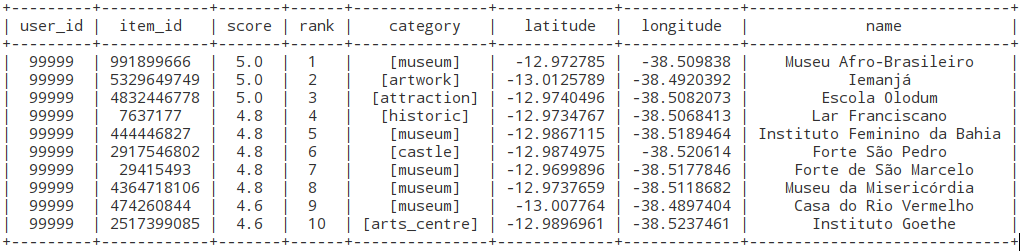
\includegraphics[scale=0.95]{images/IS_pearson_newUser_results.png}
    \caption{Exemplo de um resultado do sistema de recomendação para o novo usuário pelo modelo \textit{Item Similarity}.}
    \label{fig:IS_pearson_newUser_results_rotate}
\end{sidewaysfigure}

\begin{sidewaysfigure}
    \centering
    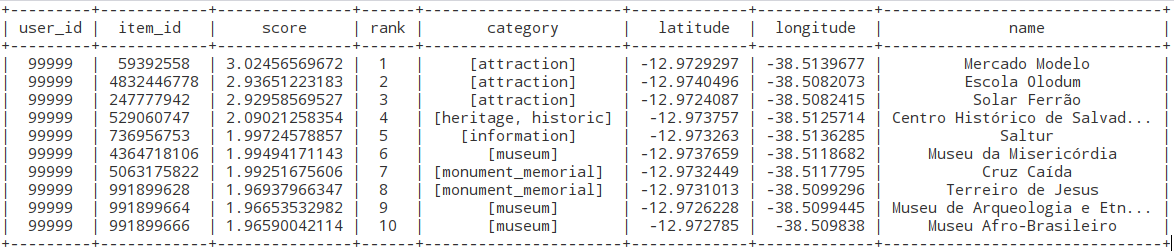
\includegraphics[scale=0.85]{images/IC-loc_item-newUser-results.png}
    \caption{Exemplo de um resultado do sistema de recomendação para o novo usuário pelo modelo \textit{Item Content}.}
    \label{fig:IC-loc_item-newUser-results_rotate}
\end{sidewaysfigure}

\begin{figure}
    \centering
    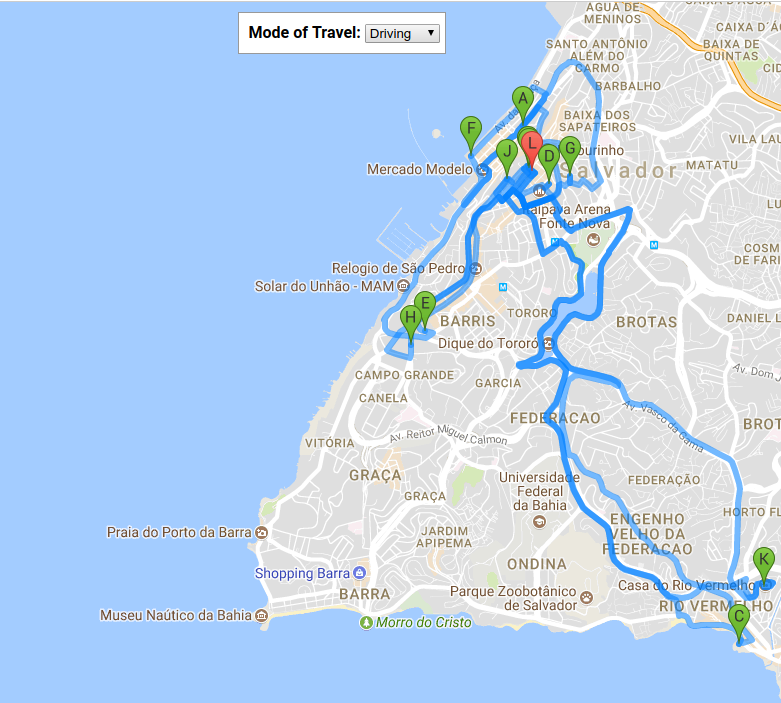
\includegraphics[scale=0.6]{images/IS_pearson-newUser-route.png}
    \caption{Exemplo de um resultado da rota para o novo usuário pelo modelo \textit{Item Similarity}.}
    \label{fig:IS_pearson_newUser_route}
\end{figure}

\begin{figure}
    \centering
    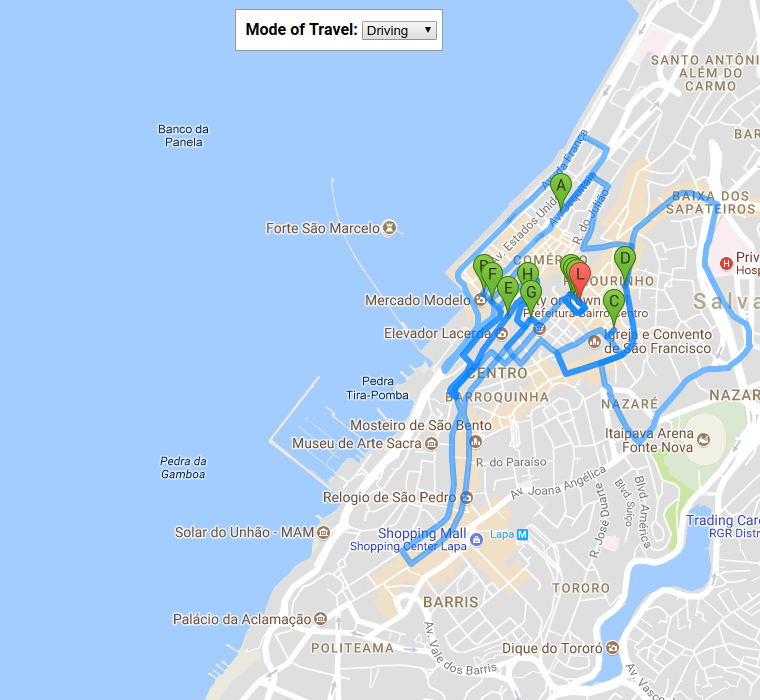
\includegraphics[scale=0.6]{images/IC-loc_item-newUser-route.png}
    \caption{Exemplo de um resultado da rota para o novo usuário pelo modelo \textit{Item Content}.}
    \label{fig:IC-loc_item-newUser-route}
\end{figure}


\section{Discussão}

Neste trabalho foi mostrado a construção de um sistema de recomendação de rotas de pontos turísticos com base em filtragem colaborativa. Em meio a tantas informações, este sistema de recomendação pode ajudar o turista que deseja conhecer pontos turísticos da cidade que está visitando mas não sabe quais pontos ir e que rota seguir.

Após analisar os resultados obtidos com as métricas utilizadas,  conclui-se que é possível fazer recomendações de acordo com as preferências do usuário e gerar rotas considerando sua origem e destino. Ainda não chega a ser um resultado bom, devido a diversos fatores, mas é algo a ponderar, analisando de que forma será possível melhorar para encontrar um modelo de recomendação que seja o ideal para este tipo de recomendação.

Além disso, este trabalho serve como um começo para serviços relacionados a área de turismo possam implementar sistemas de recomendação para os seus usuários, gerando rotas que facilitem a excursão do turista durante a sua viagem. O Apontador \footnote{https://www.apontador.com.br/}, site de busca de lugares, serviços e facilidades, pode fazer uso da abordagem proposta neste trabalho para fazer sugestão de pontos de acordo com as avaliações feitas pelos usuários que o site já tem cadastrado, além de gerar rotas de acordo com as suas preferências.

\section{Pontos de Melhoria}

Durante a realização deste projeto, houveram alguns problemas que podem ter impactado no resultado deste trabalho. Um dos principais problemas foi na obtenção de dados através da API do Google Maps. Como foi citado no capítulo 4 sobre o funcionamento do sistema \ref{sec:operation}, para fazer a busca do local no Google Places, era necessário informar o nome e a localização do ponto de interesse, o que trouxe problemas relacionados a error de grafia ou ruídos, como em casos em que naquela localização não havia um local com aquele nome, trazendo um outro local próximo. Muitos casos foram resolvidos, mais ainda é um ponto a se considerar como melhoria.

Outro problema é a limitação da quantidade de avaliações por local da API do Google Maps, impactando na quantidade de itens por usuário no banco de dados. Por conta disso, item que contém mais de 1000 avaliações, somente são considerados as cinco últimas análises. Além disso, não é disponibilizado muitas informações de usuários, impossibilitando trabalhar com modelos de recomendação voltados ao usuário.

Algo a acrescentar que pode ajudar nos futuros trabalhos é a ampliação do banco de dados para outras áreas além da cidade de Salvador. Para a realização de testes, foi utilizada somente pontos turísticos de Salvador, criando um impasse para turistas que nunca vieram a Salvador, mas já foram em outros pontos turísticos de outras regiões do Brasil mas que não etão na base de dados.

Para finalizar, o modelo \textit{Item Content} é um algoritmo recentemente implementado na ferramenta GraphLab, atualmente sendo um algoritmo no estado beta. Por conta disso, talvez alguns resultados possam ter sido prejudicado por conta de erros ou \textit{bugs} que o algoritmo possa a ter. Com tudo isso, existe ainda muitos pontos a serem melhorados e explorados, gerando novos dados, seguindo a proposta apresentada neste trabalho.

\section{Sumário}

Este capítulo apresentou os principais resultados obtidos durante o desenvolvimento dos experimentos para avaliar a implementação de um sistema de recomendação de rotas de pontos turísticos. No começo, foram apresentadas as metodologias de avaliação utilizadas no estudo, a base de dados a as métricas utilizadas. O estudo apresentado neste capítulo mostrou que é possível construir um sistema de recomendação que auxilie os turistas nas suas próximas viagens, conhecendo novos lugares de acordo com os seus interesses.